\documentclass[a4paper,10pt]{article}
\usepackage{amsmath}
\usepackage{amsthm}
\newtheorem{mydef}{Definition}
\usepackage{url, hyperref}
\usepackage{amsthm}
\usepackage{amsfonts}
\usepackage{amssymb}
\newtheorem{theorem}{Theorem}
\newtheorem{lemma}{Lemma}
%\usepackage{fullpage}
\usepackage{tikz}
\usepackage{float}
\usepackage{listings}
\usepackage{color}
\usepackage{mathtools}
\usepackage[T1]{fontenc}
\usepackage{subfigure}
\usepackage{algorithm}
\usepackage{algpseudocode}
\bibliographystyle{plain}

\newenvironment{changemargin}[2]{%
\begin{list}{}{%
\setlength{\topsep}{0pt}%
\setlength{\leftmargin}{#1}%
\setlength{\rightmargin}{#2}%
\setlength{\listparindent}{\parindent}%
\setlength{\itemindent}{\parindent}%
\setlength{\parsep}{\parskip}%
}%
\item[]}{\end{list}}

\usepackage[linecolor=green!70!white,
backgroundcolor=blue!20!white,bordercolor=red]{todonotes}
\newcommand{\note}{\todo}

\begin{document}
\begin{titlepage}

\begin{changemargin}{-1cm}{-1cm}
\begin{center}

\begin{minipage}{1.2\textwidth}
\begin{center}
\vspace{2cm}
    {\Huge \bf Efficient segmentation algorithms for shark fin
identification }
\end{center}
\end{minipage}

\vspace{1.3cm}

\begin{minipage}{0.49\textwidth}
\begin{center} \LARGE
\emph{Author:}\\
L. Cilli\'{e}, 16010450
\end{center}
\end{minipage}
\begin{minipage}{0.49\textwidth}
\begin{center} \LARGE
\emph{Project Advisors:} \\
Prof. B.M. Herbst\\Dr. S.J Van der Walt

\end{center}
\end{minipage}

\vspace{1.3cm}
{\LARGE October 2013}

\end{center}

\vfill

\vspace{20mm}
\hfill{\LARGE Honours Project, Applied Mathematics}\hfill\,

\,\hfill{\LARGE Stellenbosch University}\hfill\,

\end{changemargin}

\end{titlepage}

\begin{abstract}
This project investigates the use of various segmentation algorithms as
  part of a larger pipeline for fin identification of Great White sharks.
For this purpose, the Growcut algorithm \cite{alg} is studied in detail.
A pipeline is developed containing various algorithms that form part of the
identification process.  The pipeline can be used to compare new shark fin
images with existing images in a database, establishing whether the shark
has been seen before.  This information can be used to determine a more accurate population estimate in a specific region
and also to keep track of the shark population,
thereby assisting in the conservation of the Great White shark.
\end{abstract}

\newpage
\tableofcontents

\newpage
\section{Problem statement and motivation}
Just as humans are identified by their fingerprints, sharks have an unique
dorsal fin structure.  Identifying shark sightings is
valuable for biological and ecological research --- such information can be used to predict migration
patterns, possible habitats and also in warning people about the
  presence of sharks in a certain area.  In order to identify the sharks and to compare various shark sightings,
images of
shark fins are analysed by a computer. 
This analysis consists of identifying the edges in the image and segmenting the
foreground, the shark, from the background, the sea.
Although the images provided are of a good quality and have been cropped
to only include the fin, the
foreground and background properties can still vary significantly, making
segmentation a
non-trivial problem. Our approach consists of
evaluating (by means of a computer) different methods for classifying foreground
and background, as well as segmenting the foreground successfully.  \\

The project was conceived by a PhD
student in Marine Biology, Ms. S. Andreotti, who approached Dr. S.J. van der Walt for
help regarding a problem she encountered in her research, namely
how images of shark fins  can be used in identifying sharks, so that their
ecological and behavioural patterns can be studied more easily.
For this purpose, a database of shark fin images had already been compiled.
To
draw reliable conclusions about the behaviour of sharks, images in the
database must be in a form such that it can be compared to new images.
The goal is to group images of an individual shark together.  We
already know that it is possible to categorize each image, because a
  person is able to group images based on the unique shape of the
dorsal fin.  To do so, one would have to find a way to match new
input data with existing images in the database, but to perform such a
  process manually is laborious. 
Since the student's 
focus is on the distribution and movements of sharks and not on developing new
software, an algorithm that automates the task makes a significant contribution. \\

Using such non-invasive methods, the Great White shark population and migration
patterns can be studied in a way that is not harmful to
the sharks, since the sharks need not to be tagged manually, thereby
contributing in their conservation and the environment.  

\newpage
Below are a few examples from the database \footnote{I am indebted to
  Ms. S. Andreotti for providing us with a sample from her carefully
    curated set of photos used in this research project.}.  
The database consists of various shark fin images, taken on different dates and
at different locations.
Also note that some sharks are
  represented more than once, i.e. the database
might contain two or more images of the same shark.

\begin{figure}[H]
\centering
\mbox{\subfigure[]{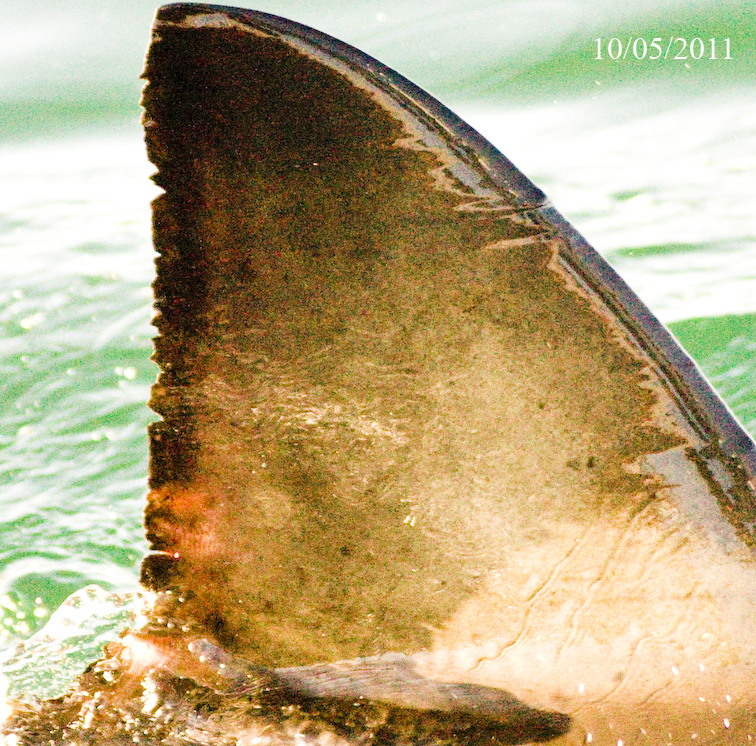
\includegraphics[width=1.5in]{haai1.jpg}} \quad
\subfigure[]{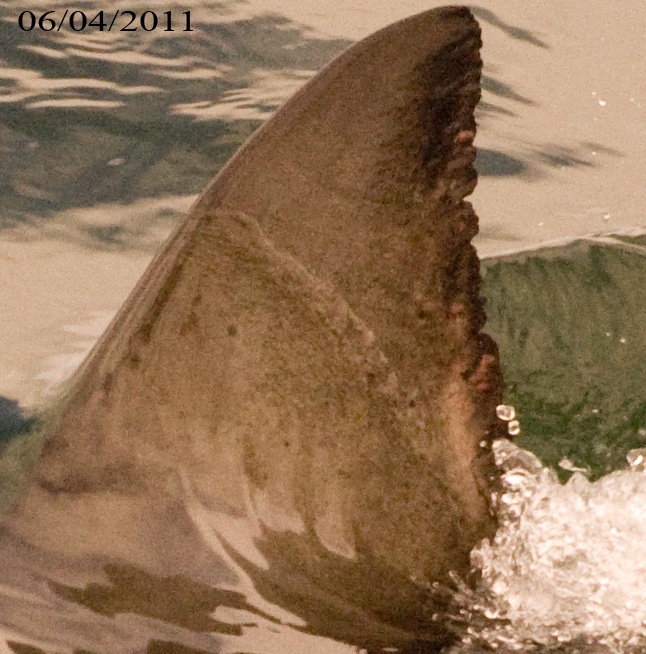
\includegraphics[width=1.5in]{haai4.jpg}} \quad
\subfigure[]{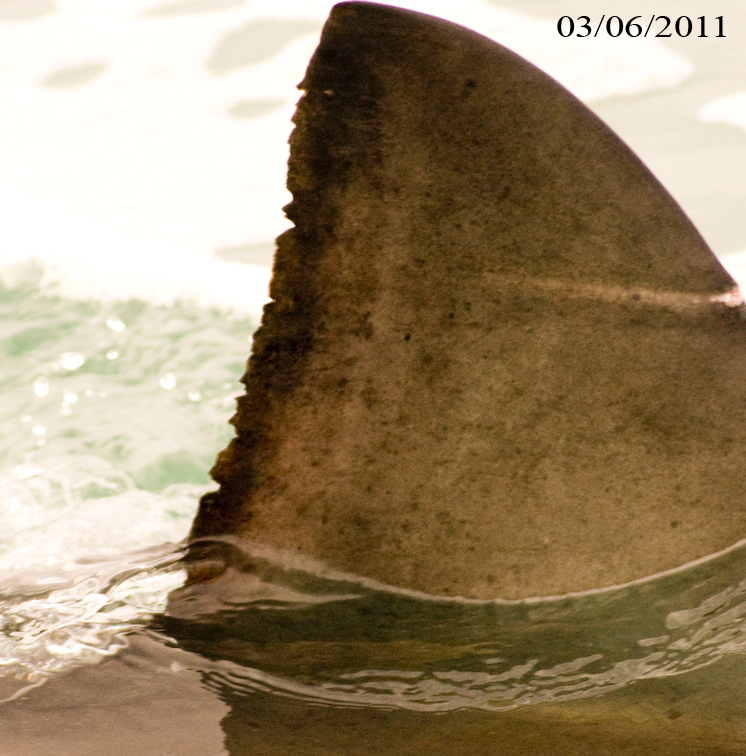
\includegraphics[width=1.5in]{haai2.jpg}}}
\end{figure}

\begin{figure}[H]
\centering
\mbox{\subfigure[]{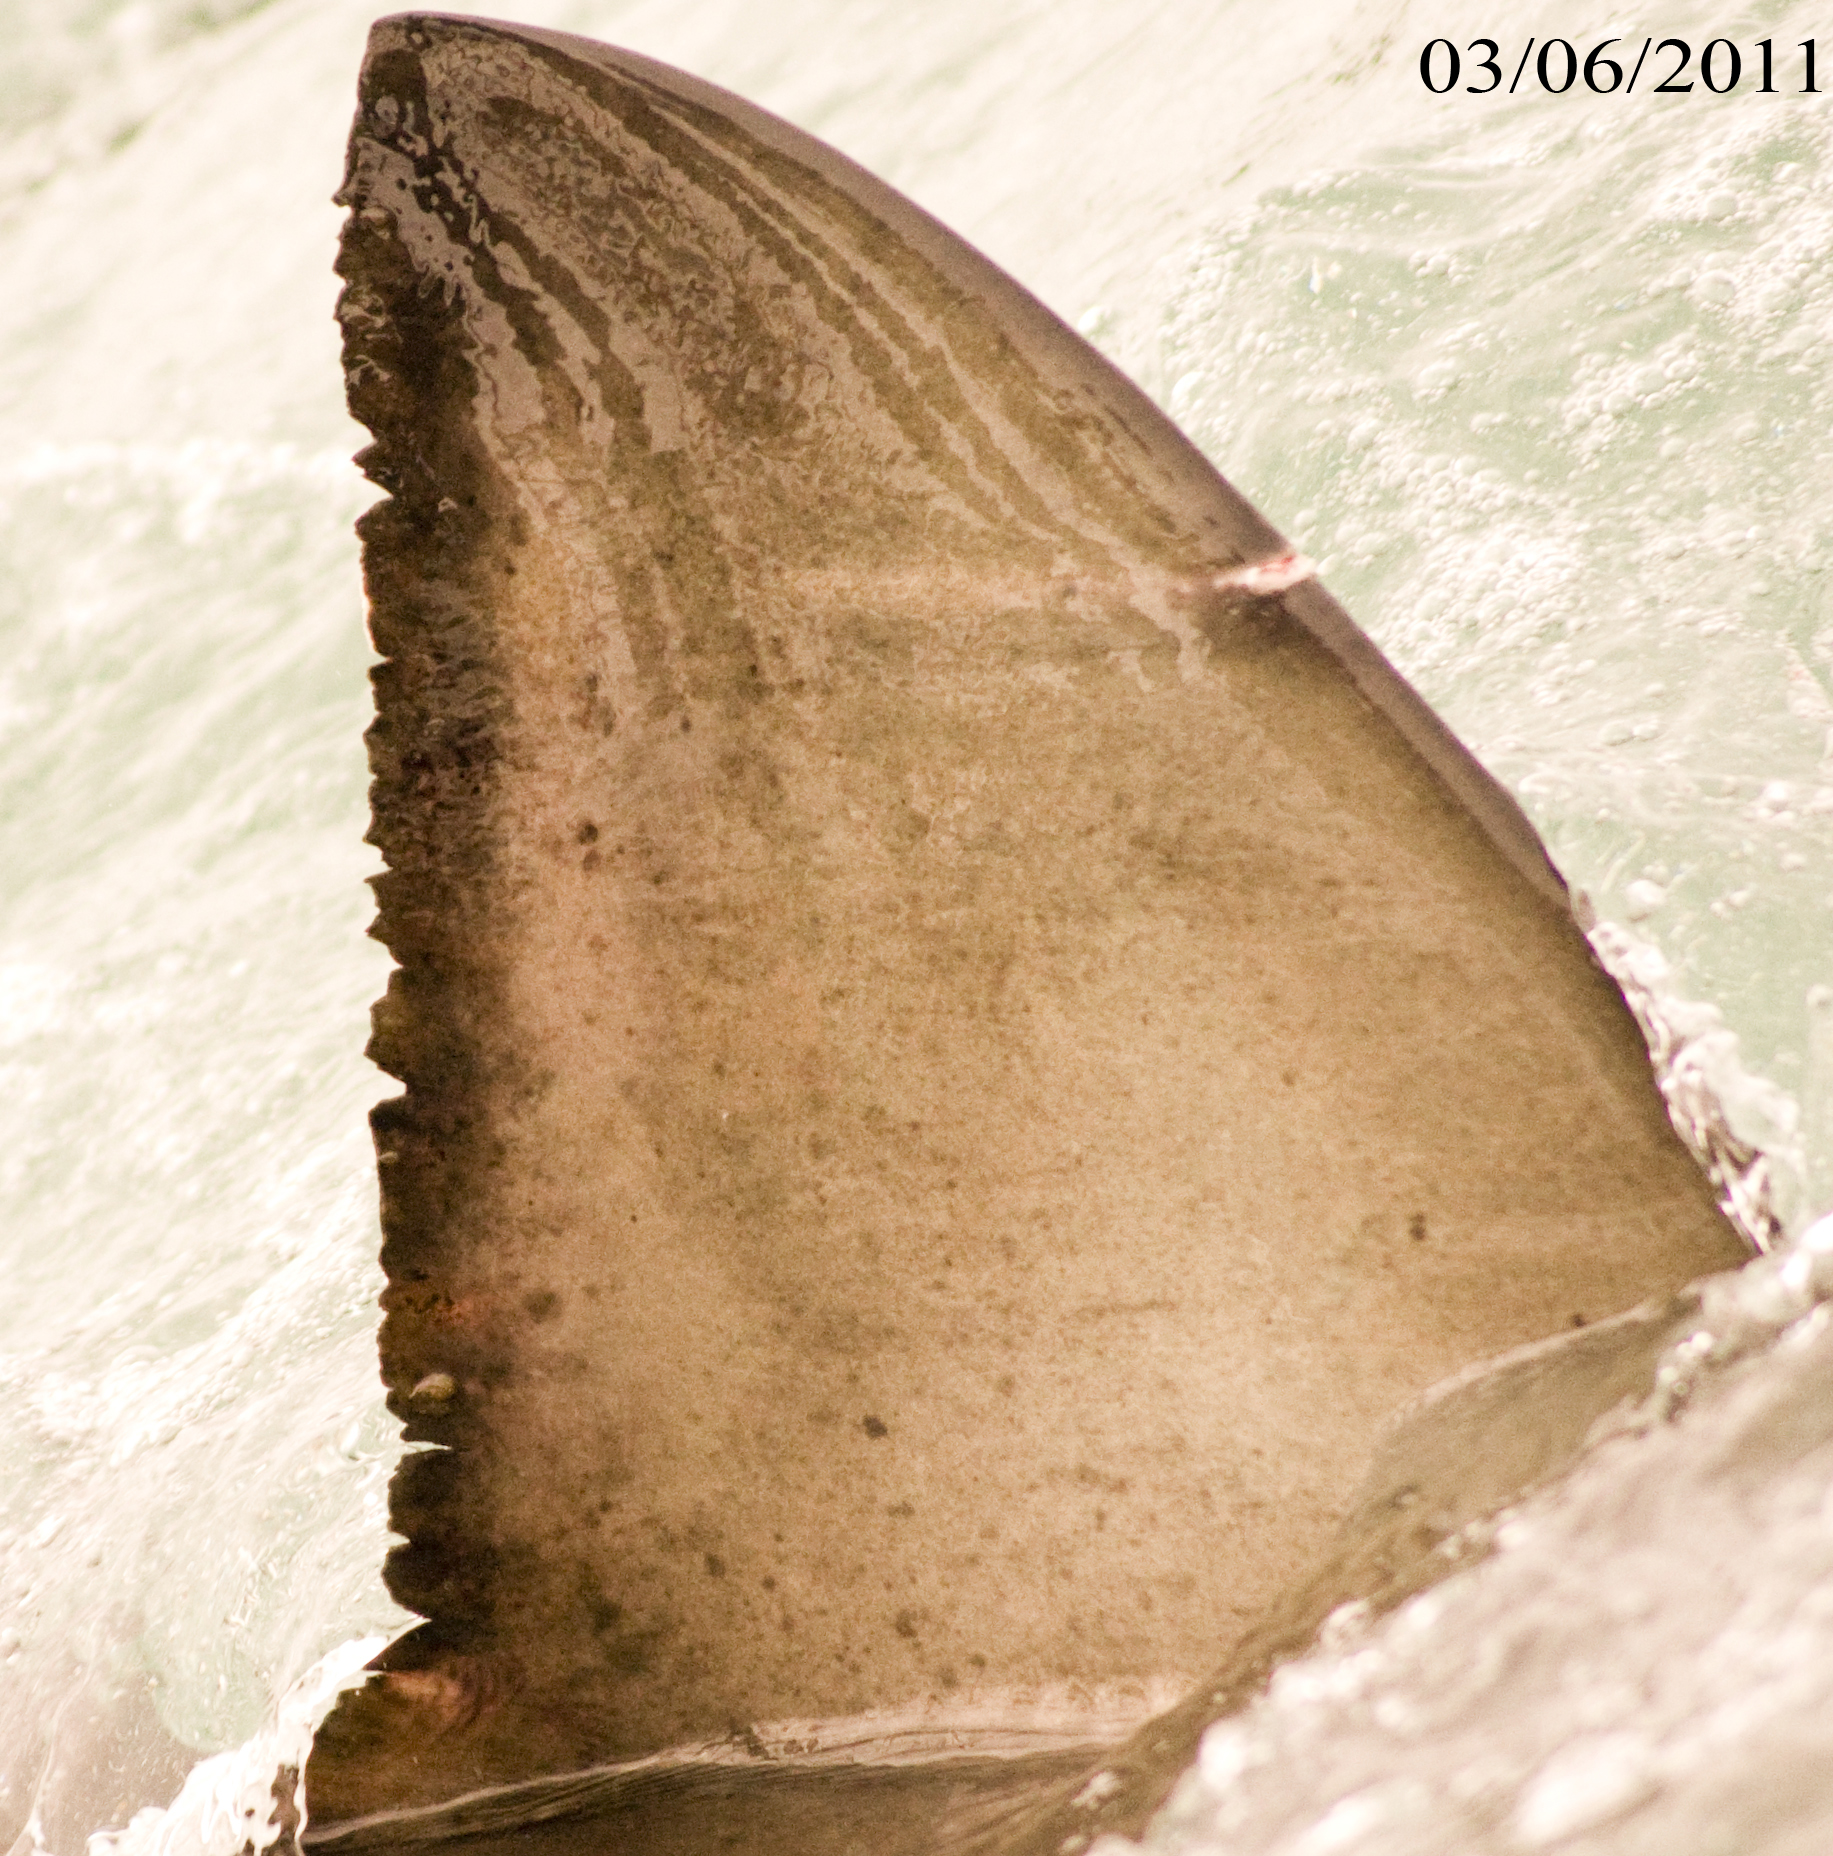
\includegraphics[width=1.5in]{haai3.jpg}} \quad
\subfigure[]{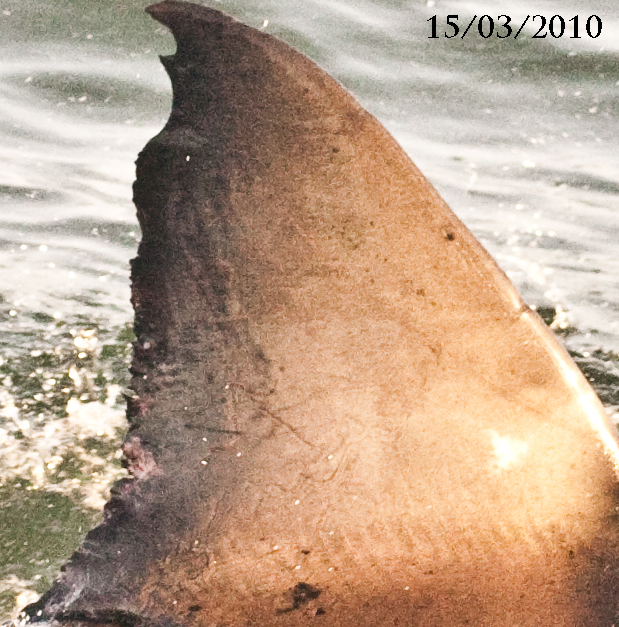
\includegraphics[width=1.5in]{haai5.jpg}} \quad
\subfigure[]{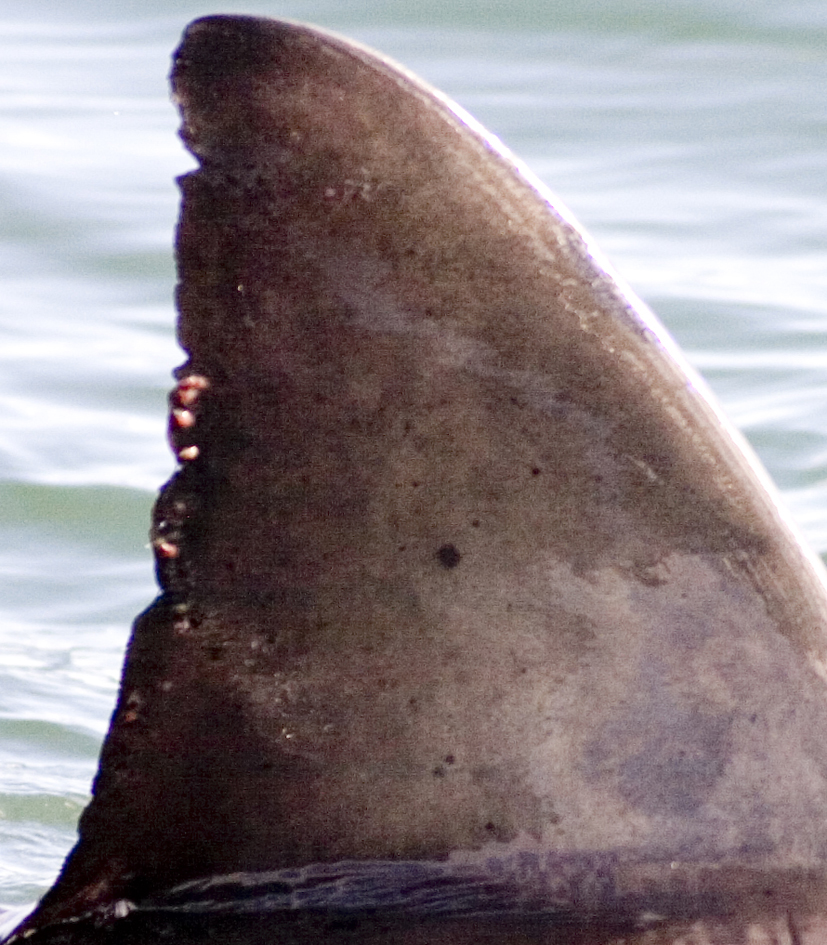
\includegraphics[width=1.5in]{haai6.jpg}}}
\end{figure}

\begin{figure}[H]
\centering
\mbox{\subfigure[]{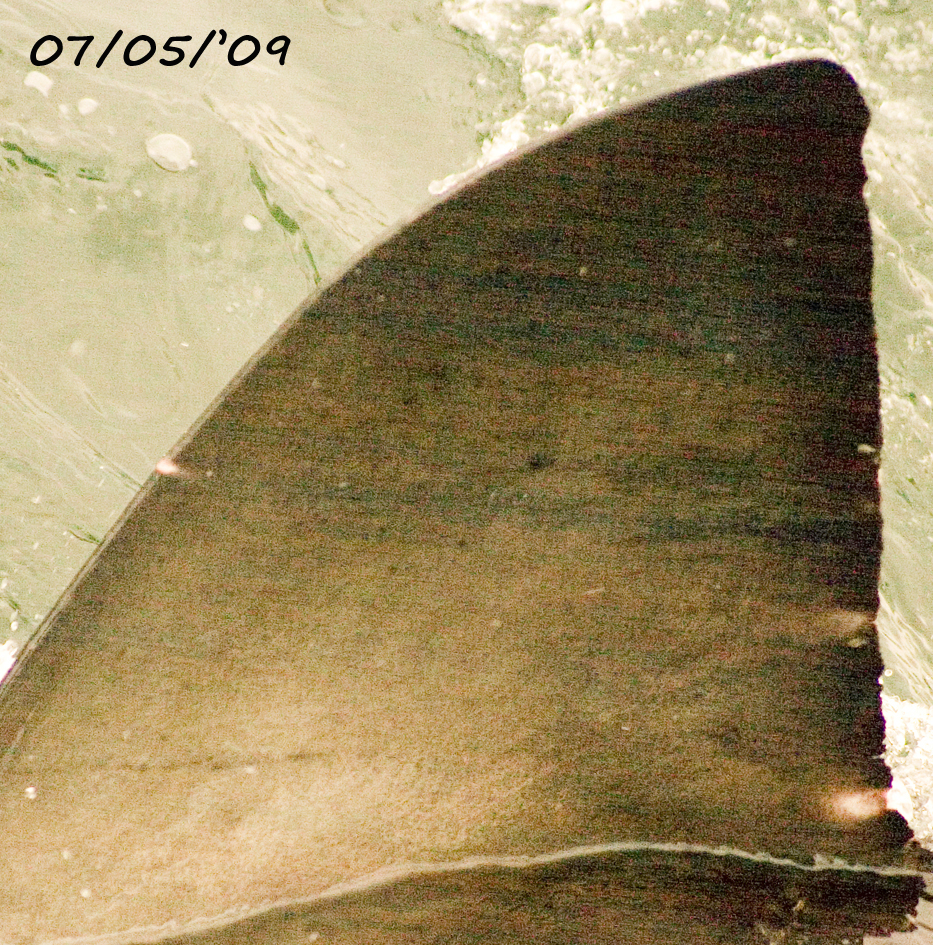
\includegraphics[width=1.5in]{haai7.jpg}} \quad
\subfigure[]{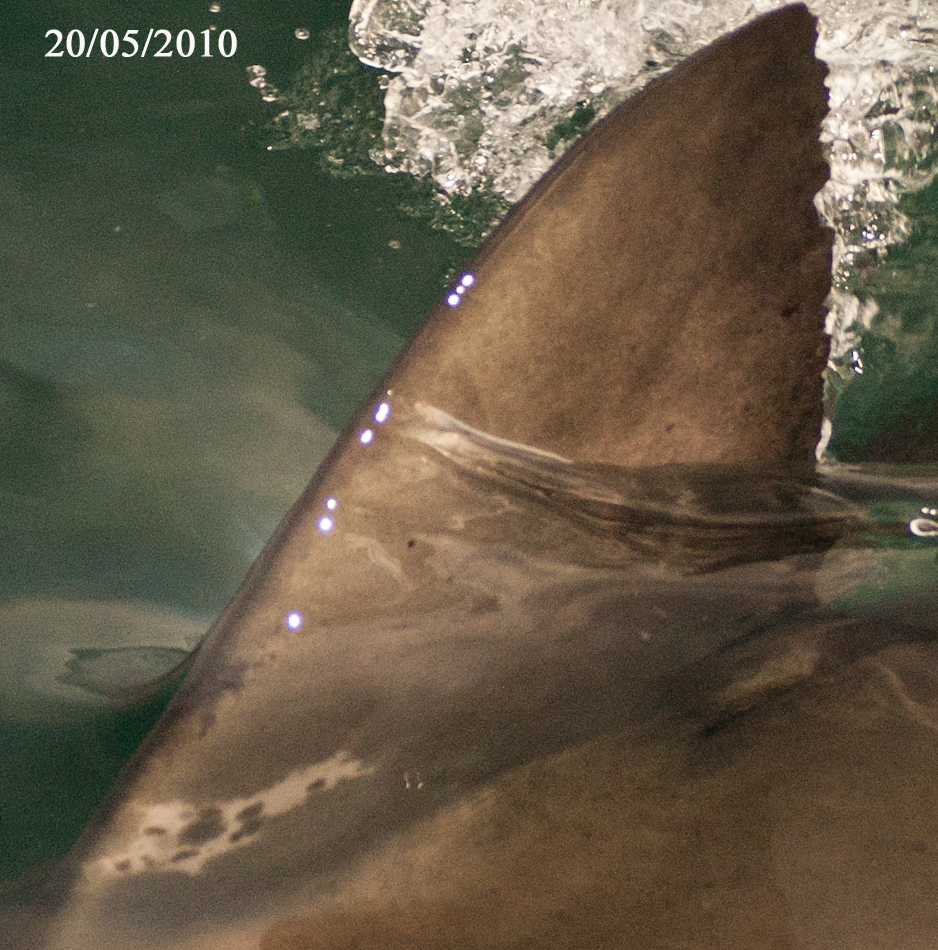
\includegraphics[width=1.5in]{haai8.jpg}} \quad
\subfigure[]{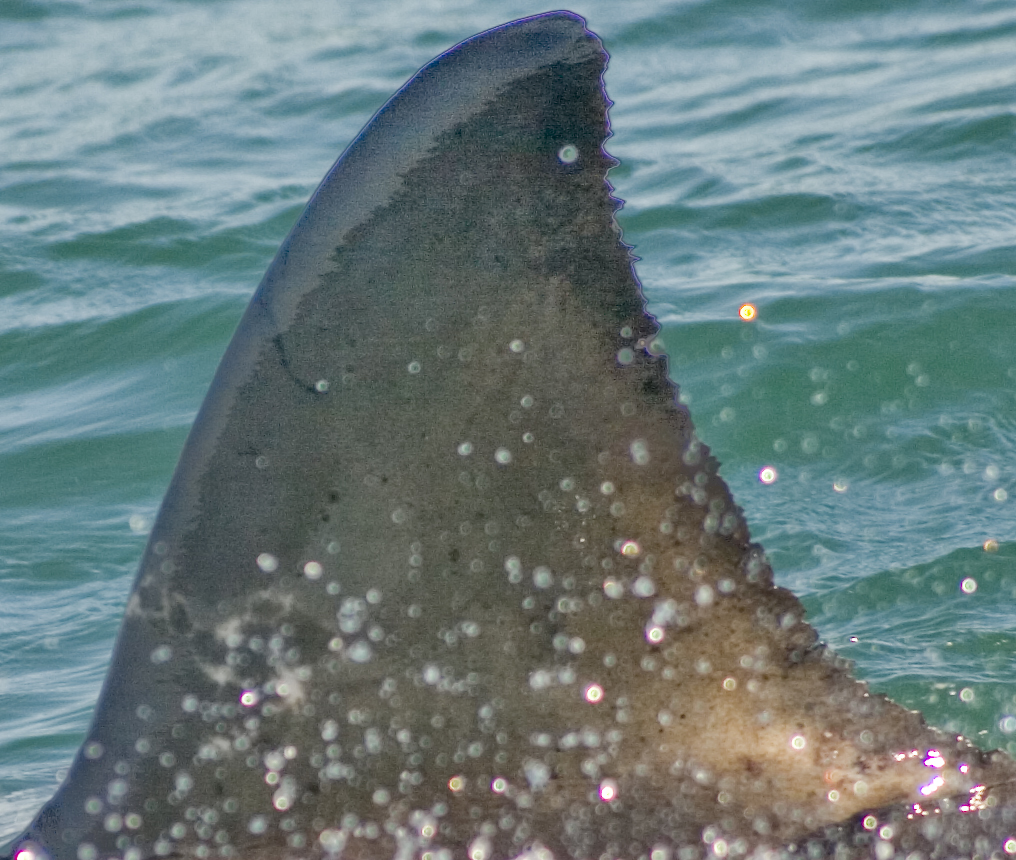
\includegraphics[width=1.5in]{haai9.jpg}}}
\end{figure}


\subsection{Background}
Image segmentation is commonly applied in image processing; it
aims to partition a digital image into multiple segments, where each
  segment consists of pixels related by some criteria.
The image can then be interpreted using a smaller number of
well-defined components as opposed to a large array of unrelated pixels \cite{segmentation}.  
In other words each pixel is assigned a label and all the pixels with the same
label share a certain
property, making the image easier to analyse. Image segmentation is
typically used to locate an object or boundaries in an image. \\

Segmentation algorithms can be classified as either supervised, meaning that
it requires user interaction, or unsupervised, meaning that it is totally
automatic.  Segmentation is a complex problem since computers must segment
an
image having only limited information about colour and space, for
example.
Supervised segmentation requires user input and interpretation which is subjective.  
On the other hand,
unsupervised algorithms need predetermined information and assumptions to work
automatically. \\

Well known examples where image segmentation is used are
for locating tumours from medical images, face and
fingerprint recognition and also in video surveillance.  See Figure \ref{examples} for illustrations.

\begin{figure}[H]
\centering
\mbox{\subfigure[]{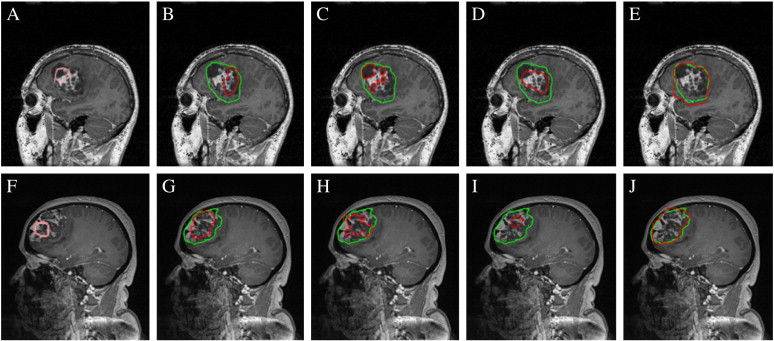
\includegraphics[width=2in]{braintumor.jpg}} \quad
\subfigure[]{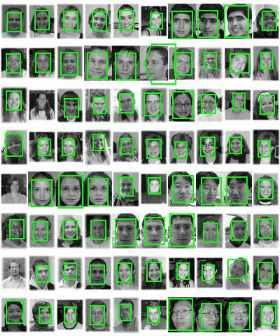
\includegraphics[width=2in]{face.jpg}}}
\caption{Image segmentation in various fields.}
\label{examples}
\end{figure}

Evaluating the segmentation outcome proves challenging.  It would be helpful to have a way of comparing
different
segmentation methods so that we know if progress is being made. 
The Berkeley Segmentation Dataset and Benchmark \cite{dataset} contains 12 000 hand-labelled
segmentations of 1 000 Corel dataset images by 30 human subjects. 
This can be used to compare human versus computer analysis of accurate segmentation. \\

Below is an example of a colour image in the Berkeley Segmentation Dataset.  The image in the middle shows the machine segmentation and the
image on the right the human segmentation.

\begin{figure}[H]
\centering
\mbox{\subfigure[]{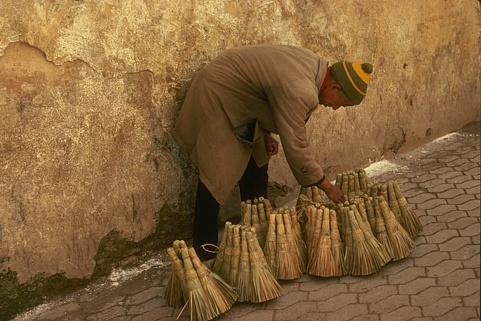
\includegraphics[width=1.5in]{data.jpg}} \quad
\subfigure[]{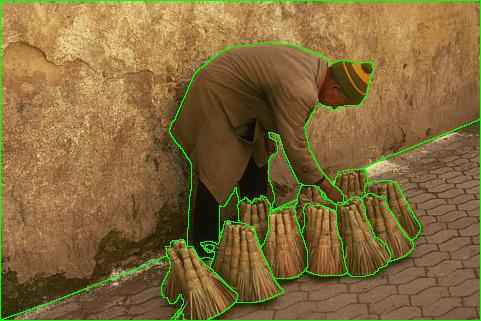
\includegraphics[width=1.5in]{data1.jpg}} \quad
\subfigure[]{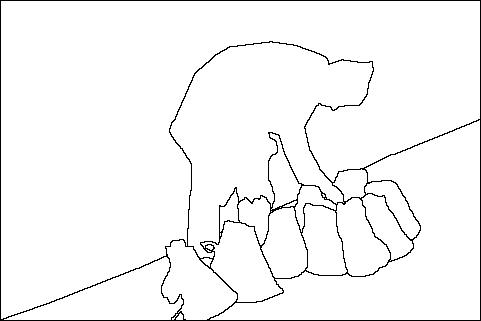
\includegraphics[width=1.5in]{data2.jpg}}}
\end{figure}

\subsection{Software -- Python}
For the purpose of this research project, the Python programming language is
used because of its simplicity, the powerful set of tools
available, and that it is easy to learn and understand.  Python is
also free to use and runs on multiple platforms.  For numerical and
scientific computations, Numpy and SciPy were used.
To improve the running time of implemented algorithms, Cython was used.  It is a
language that compiles to a Python extension module and a superset of the
Python language that allows calling C-functions and declaring C-types on
variables and class attributes.  This
results in the generation of efficient C-code from Cython code.
Scikit-image was used to investigate various image processing
techniques. \\

To ease collaboration, GitHub was used.  Github is a web-based hosting service
for software development projects.  This allowed us to easily
share code and documents and also quickly obtain feedback.
Figure \ref{packages} depicts the various software packages used in this research project.

\begin{figure}[H]
 \centering
 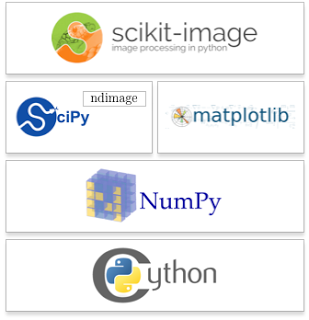
\includegraphics[width=3in]{logos.jpg}
 \caption{Various packages used in this research project.}
 \label{packages}
\end{figure}

In the next section the development of a pipeline for shark fin identification is discussed.

\newpage
\section{Overview of pipeline}
The procedure of identifying sharks can be
  divided into several components, together forming an image processing pipeline, each implemented as part of
  a bigger pipeline.  Below is a diagram showing the structure of the pipeline.  The first algorithm is an orientation detection
algorithm that will determine whether the shark fin is orientated to the left or the right in the image.
Then a segmentation algorithm will segment the shark fin from the image such that the path that defines the shark fin 
can easily be detected by the fin detection algorithm.  Thereafter a dynamic time warping algorithm is used
to compare the the paths that describe the fins and to see how shark fins in the database compare.

\begin{figure}[H]
 \centering
 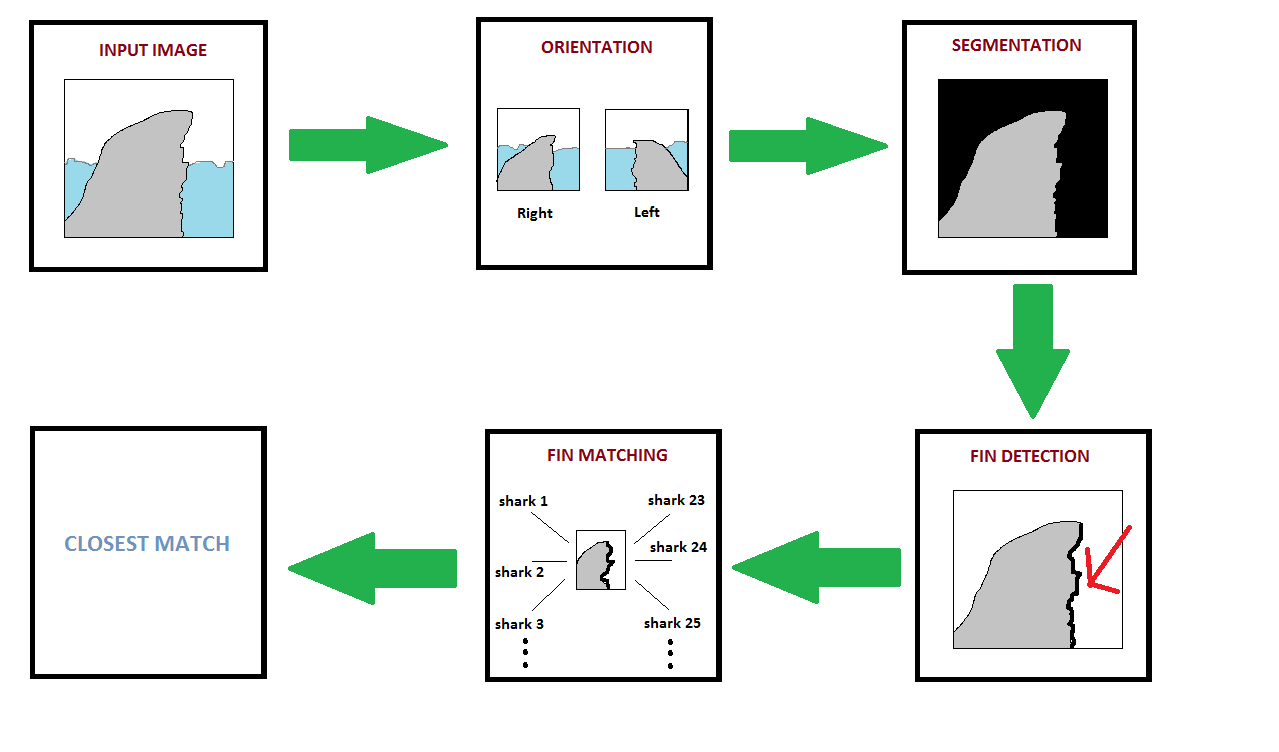
\includegraphics[width=5in]{pipeline.png}
\end{figure}

The various algorithms will now be discussed in detail.  

\subsection{Orientation}
\label{orient}
To provide a consistent basis for further analysis, the
orientation of the shark fin in the image is determined as the direction in
which the shark is
swimming.  The images are flipped so that
all the shark fins have the same direction.  This will assist in specifying the vertices of the relevant polygons when performing
segmentation.
The method of Principal Components Analysis (PCA) is used to determine the orientation of the shark fin.  When applying
PCA, we are interested in finding the direction of maximum variation in the
data, the pixel values in the shark fin images.  Suppose we have $K$, $n$-dimensional, data points, $\mathbf{x}_k,$ for
$k=1,2, \ldots ,K$.  A covariance matrix, $C$, is computed from our shark fin image as 
\[
 C_{\mathbf{x}} = \frac{1}{K} \sum_{k=1}^{K} \mathbf{x}_{k}\mathbf{x}_{k}^{T} -
\mathbf{m}_{\mathbf{x}}\mathbf{m}_{\mathbf{x}}^{T} 
,\]
where
\[
 \mathbf{m}_{\mathbf{x}} = \frac{1}{K} \sum_{k=1}^{K}\mathbf{x}_{k}
\]
is the mean of the data, computed along the columns of the shark fin image as an array. \\


From $C$, the eigenvalues and eigenvectors are determined, which will indicate the
variance and principal directions respectively.
The direction of the eigenvector corresponding to the largest eigenvalue will
then indicate the orientation of the shark fin. \\

Below is a dummy shark fin image where the orientation is detected using PCA.
Note the principal axis, largest eigenvector, in blue, which gives the
orientation of the shark fin.
\begin{figure}[H]
 \centering
 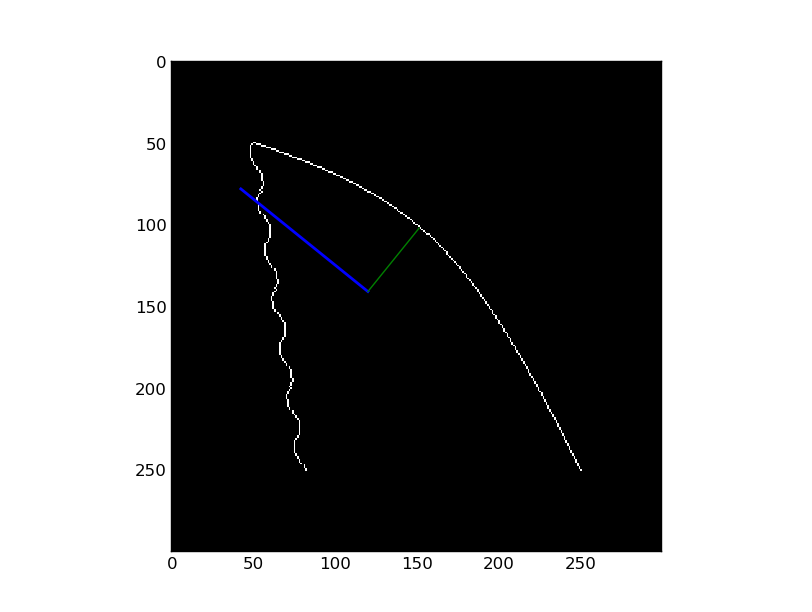
\includegraphics[width=4in]{orientation.jpg}
 \caption{Orientation of the shark fin detected by means of PCA.}
 \label{orientation}
\end{figure}

A Sobel filter is applied 
to identify prominent edges in the image.  After identifying the prominent edges
, a threshold is applied , using Otsu's method, to convert the image into a binary image.
PCA can now be done on
the image to determine the principal axes of edge pixels.  If the gradient
of the line defining the principal direction lies between 0 and
$\frac{\pi}{2}$ radians, the orientation of the shark fin is
identified as
"right", otherwise the orientation is identified as "left". 

\subsection{Segmentation}
\label{segmentation}
The task is to separate the foreground, the shark fin, from the background,
the sea.  For this purpose, the region growing segmentation algorithm,
Growcut (see \ref{growcut}) is used.  Growcut requires the user to specify a few
foreground and background pixels from which the growing can be
initiated. The Growcut
  algorithm is discussed in detail in \ref{growcut}.
Initially this was done by first determining the orientation of the fin (see
\ref{orient}) and then specifying a few pixels according to its orientation, see 
\ref{segmentation}.  \\

\begin{figure}[H]
 \centering
 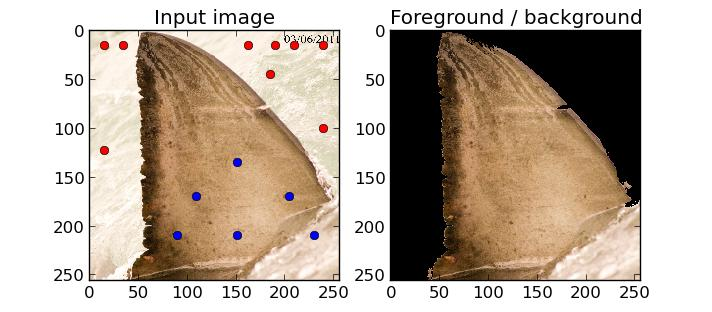
\includegraphics[width=5in]{segmentation.jpg}
 \caption{Growcut segmentation on a shark fin image by selecting a few
foreground and background pixels, shown in blue and red respectively.}
 \label{segmentation}
\end{figure}

The specification of
the foreground and background pixels is done using the function
\texttt{grid\_points\_inside\_poly()}\cite{scikit} from the \texttt{morphology} module in
\texttt{scikit-image}.  This function selects all points inside a given
polygon.  These selected  points are then set as the initial foreground and background pixels
respectively (see
Figure \ref{segmentation1}).
Since the images in the database, and images in general, are not
all the same size, the corners of the polygon are specified according to the size
of the image.  This then makes it work consistently across images of different sizes.  \\

\begin{figure}[H]
 \centering
 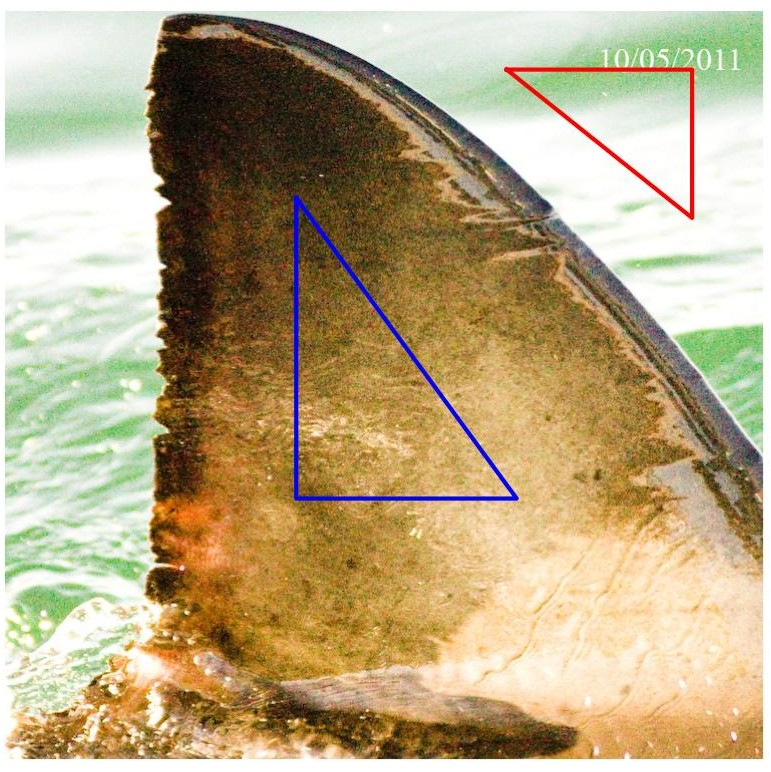
\includegraphics[width=2.6in]{polyshark.jpg}
 \caption{Growcut segmentation on a shark fin image by selecting all points in a
given polygon as foreground and background pixels, shown as blue and red
 polygons respectively.}
 \label{segmentation1}
\end{figure}

Now that we have specified a few foreground and background pixels, we also
need to specify the size of the neighbourhood around cells when the algorithm
is 'growing' as well as the number of iterations the algorithm should follow.
These parameters inevitably influence the success of the
segmentation. \\

Below is an example of the final output of the segmentation process. \\

\begin{figure}[H]
 \centering
 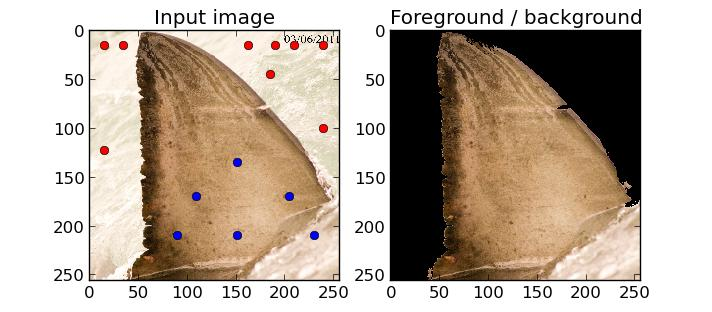
\includegraphics[width=5in]{segmentation.jpg}
 \caption{Segmented shark fin image.}
 \label{segmentation1}
\end{figure}

At the moment the segmentation algorithm is time consuming to execute.
This slows down the whole process of identification.  Repeated calculations of the
  same segmentation can be avoided by caching, 
or the segmentation process can be left out.  The latter will then result in
finding the path defining the fin directly from the edge image, keeping 
in mind that we will then have to find a different way of identifying the
  actual segment that belongs to the fin itself.

\subsection{Fin detection}
The objective is to identify the serrated part of the dorsal shark fin. In order
to, do this, we need to extract this part of the fin, in such a way that it can be 
compared with other fins easily.
We use the
Sobel operator,
well-known in edge detection, to identify edges in the image.
The Sobel operator is a discrete differential operator that approximates the
gradient of the image intensity function.  It uses two different $3 \times 3$
masks, $M_x$ and $M_y$, which are convolved with the original image to
approximate the
derivatives, both in the horizontal $x$-
and the vertical $y$-directions.  \\

Define $A$ as the input image and $G_x$ and $G_y$ as the gradient images in the
$x$-and $y$-direction respectively,
after convolving with $A$.  $M_x$ and $M_y$ is given by

\[
 M_x = \begin{pmatrix*}
        1 & 0 & -1 \\
        2 & 0 & -2 \\
        1 & 0 & -1
       \end{pmatrix*}
\mbox{ , }
 M_y = \begin{pmatrix*}
        1 & 2 & 1 \\
        0 & 0 & 0 \\
        -1 & -2 & -1
       \end{pmatrix*}
.\]

At each point in the image, the gradient approximations can be combined to give
the gradient magnitude image, calculated  as
\[
 G = \sqrt{G_x^2+G_y^2}
.\]

The Sobel operator applied to one of the shark fin images is shown in Figure 
\ref{sobel}.
We can see the edge of the fin in the $G$ image on the right clearly
identified.

\begin{figure}[H]
 \centering
 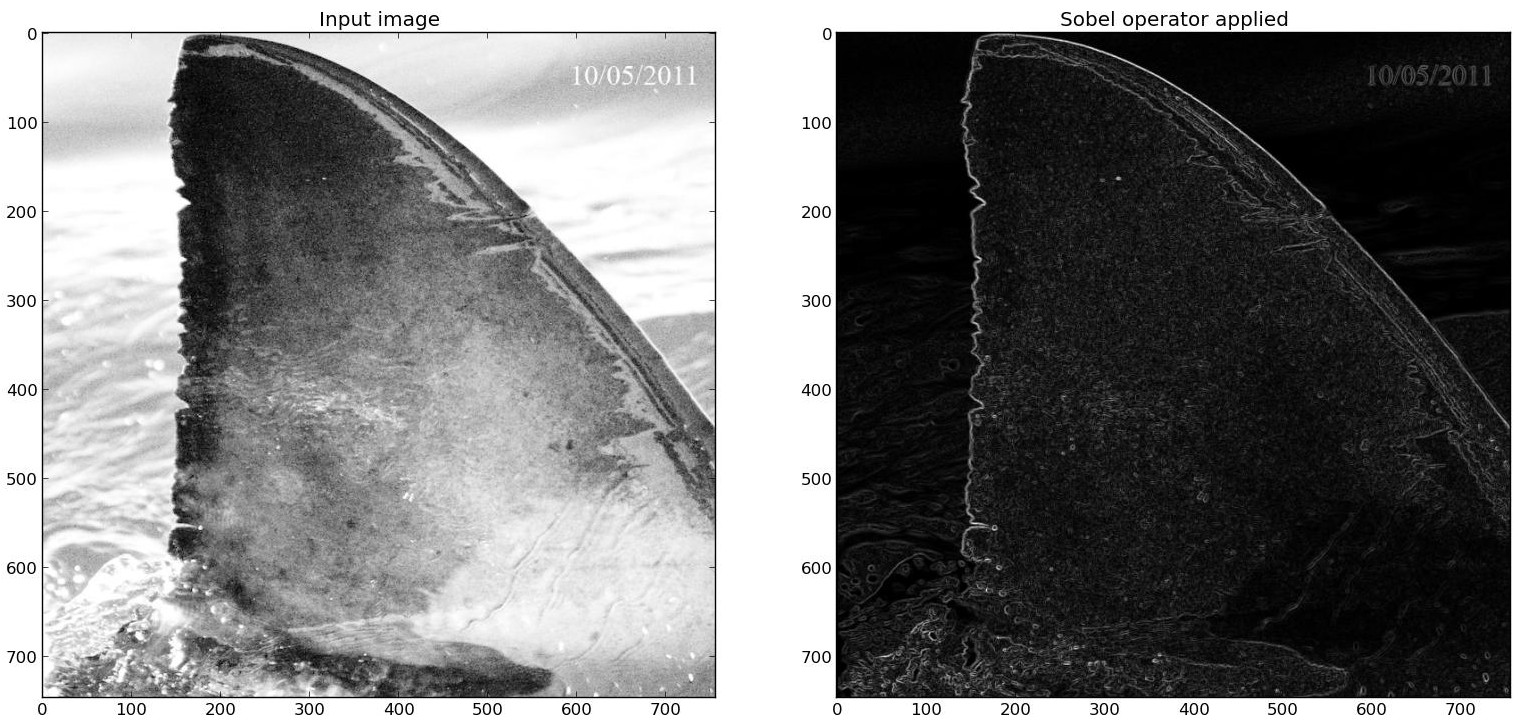
\includegraphics[width=5in]{sobel.jpg}
 \caption{The Sobel operator.}
 \label{sobel}
\end{figure}

The next step is to extract only the unique part of the fin needed for
identification.   This is done by first inverting the edges and then squaring
them to increase their weight and thereby making them more prominent.  We make use of a function 
\texttt{route\_through\_array()}\cite{scikit} from the \texttt{graph} module in scikit-image.
 This function enables us to find a lowest cost path through the
 image.
Since we are working on the segmented image, we allow any start and end point
for the path by setting the first and last rows of the
  cost matrix = 0.  All
pixel coordinates running on the edges of the image is then removed from the
path.  It is known that the fin itself becomes less well defined when moving towards its bottom part,
and then there is the
  bottom flappy part of the fin which can move between subsequent images.
  Ideally, we should make the bottom part count less than the top by only using the top
$\frac{2}{3}$ of the fin for comparison.\\

In Figure \ref{fin} an example of the path, in blue, that was detected on the shark
fin is shown.
\begin{figure}[H]
 \centering
 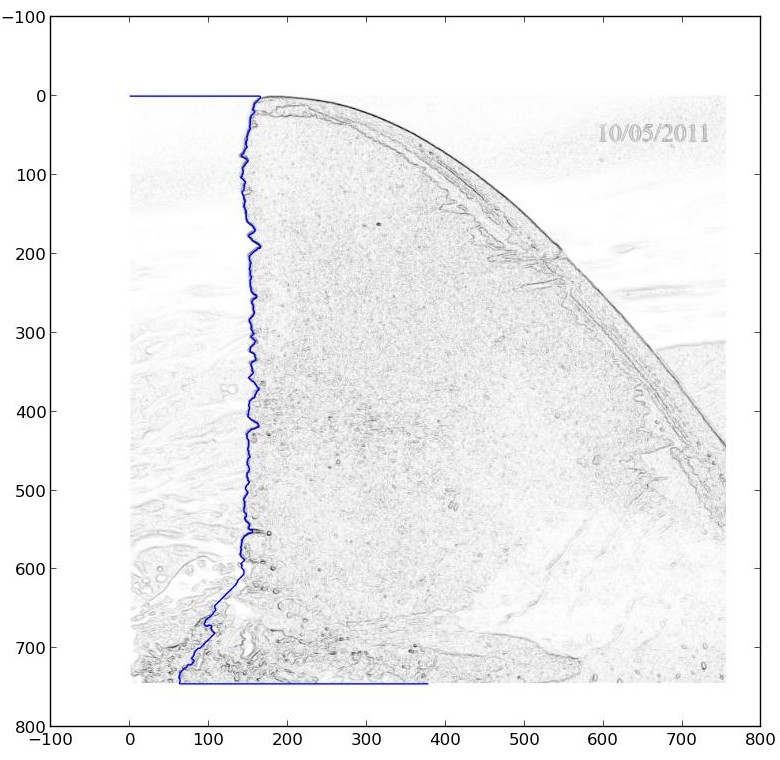
\includegraphics[width=3in]{path.jpg}
 \caption{Fin path detected.}
 \label{fin}
\end{figure}

Images such as the one in Figure \ref{shadow} below pose a challenge when finding the path defining the dorsal fin.
Since the reflection of the fin on the water is so prominent, the path which is detected by this algorithm also
picks up the reflection.  We are therefore unsure
where the path starts and ends.  This can be corrected either by
making sure the reflected part will be segmented out as background during the segmentation process or by
moving the detected path over the shark fin image and detecting drastic changes in pixel
values.  These changes will then indicate the starting point and end point of the path.

\begin{figure}[H]
 \centering
 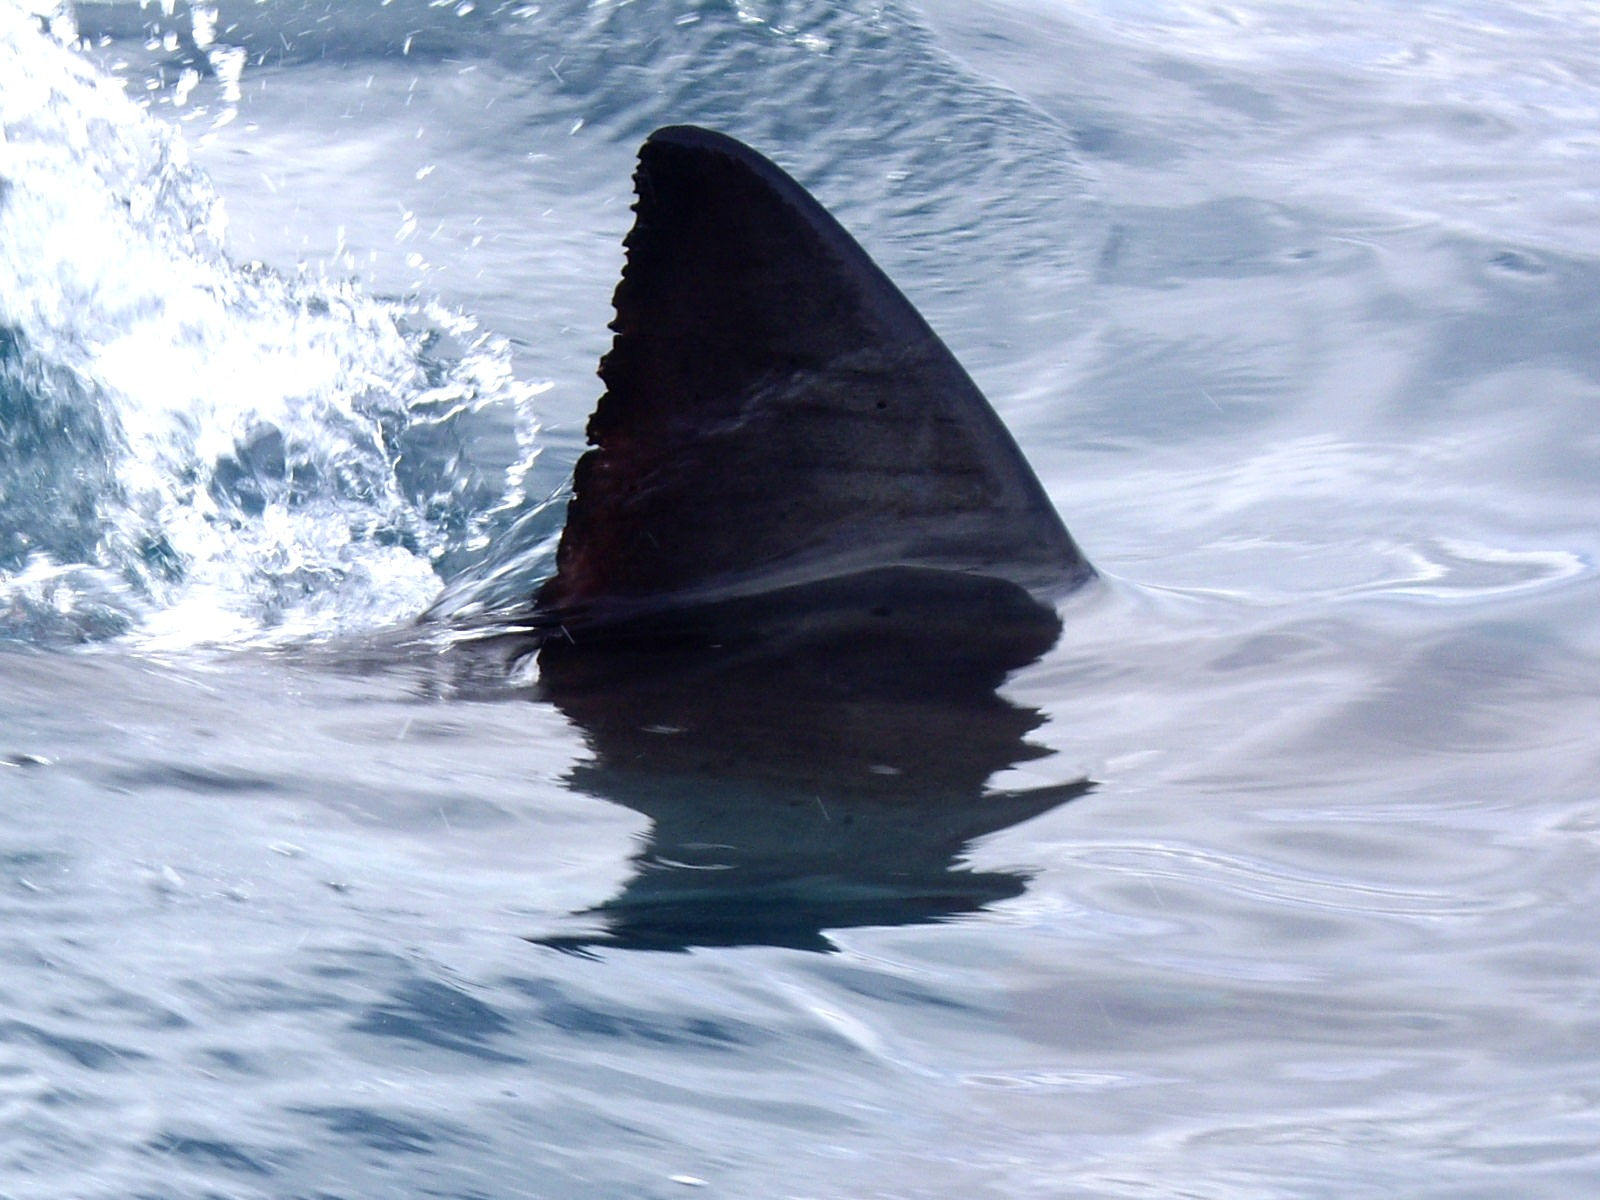
\includegraphics[width=3in]{reflectfin.jpg}
 \caption{The prominent reflection of the dorsal fin in the water.}
 \label{shadow}
\end{figure} 

\subsection{Fin matching}
Dynamic time warping (DTW) is an algorithm used for
measuring the similarity between two similar sequences which may vary in time or
speed.  It differs from linear comparison in the
sense that it accommodates sequences of different lengths, warping the
sequences for the best fit to be compared.
Any data that can be represented linearly can be analysed using DTW.  \\

When comparing two sequences, a typical approach is to calculate the distance
between corresponding points. A point-wise comparison with the Euclidean
metric can be done, whereas that will not work for varying length, time warped sequences.  But since the sequences
need not be the same length, we will make use of a non-linear
alignment. \\

Some preprocessing needs to be done and involves the following.
The DTW implementation\footnote{I am indebted to
  Dr. S.J. van der Walt for providing us with an implementation.} we use, only accomodates
sequences that do not vary in length by more than $50\%$. In our case, there are sequences
that do not satisfy this constraint.  The reason for this is because the images are not all the same size.
Theoretically, the images can be scaled, but that poses the risk of losing important features of the fin in the image.
For that reason, we rather apply interpolation on the shorter sequence, 
 such that its length is at least $75\%$ of the length of the longer sequence. 
 
Another challenge we are faced with is the fact that fins corresponding to the 
same shark might not be orientated with the same gradient in the images.  
We show an example in Figure \ref{gradient}.  \\
 
\begin{figure}[H]
\centering
\mbox{\subfigure[]{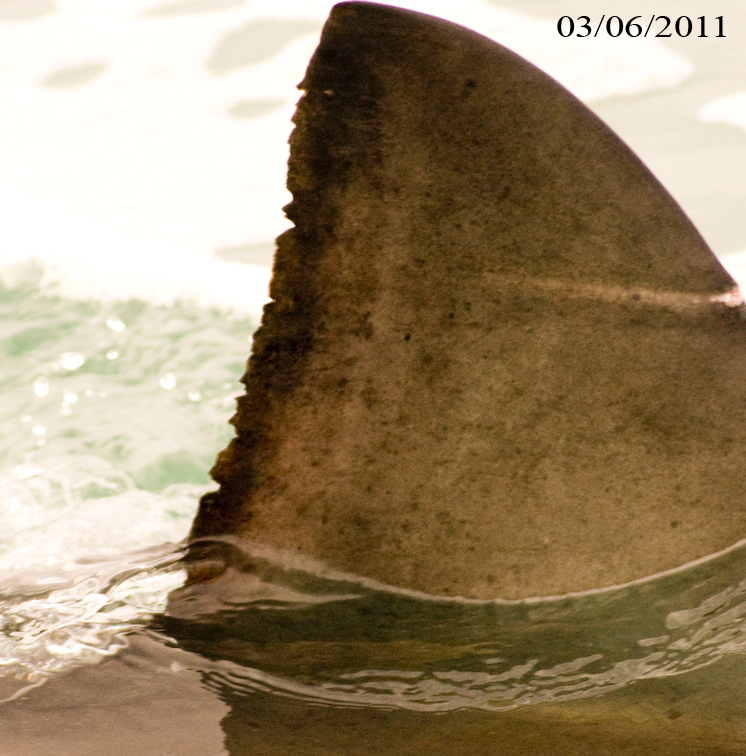
\includegraphics[width=2in]{haai2.jpg}} \quad
\subfigure[]{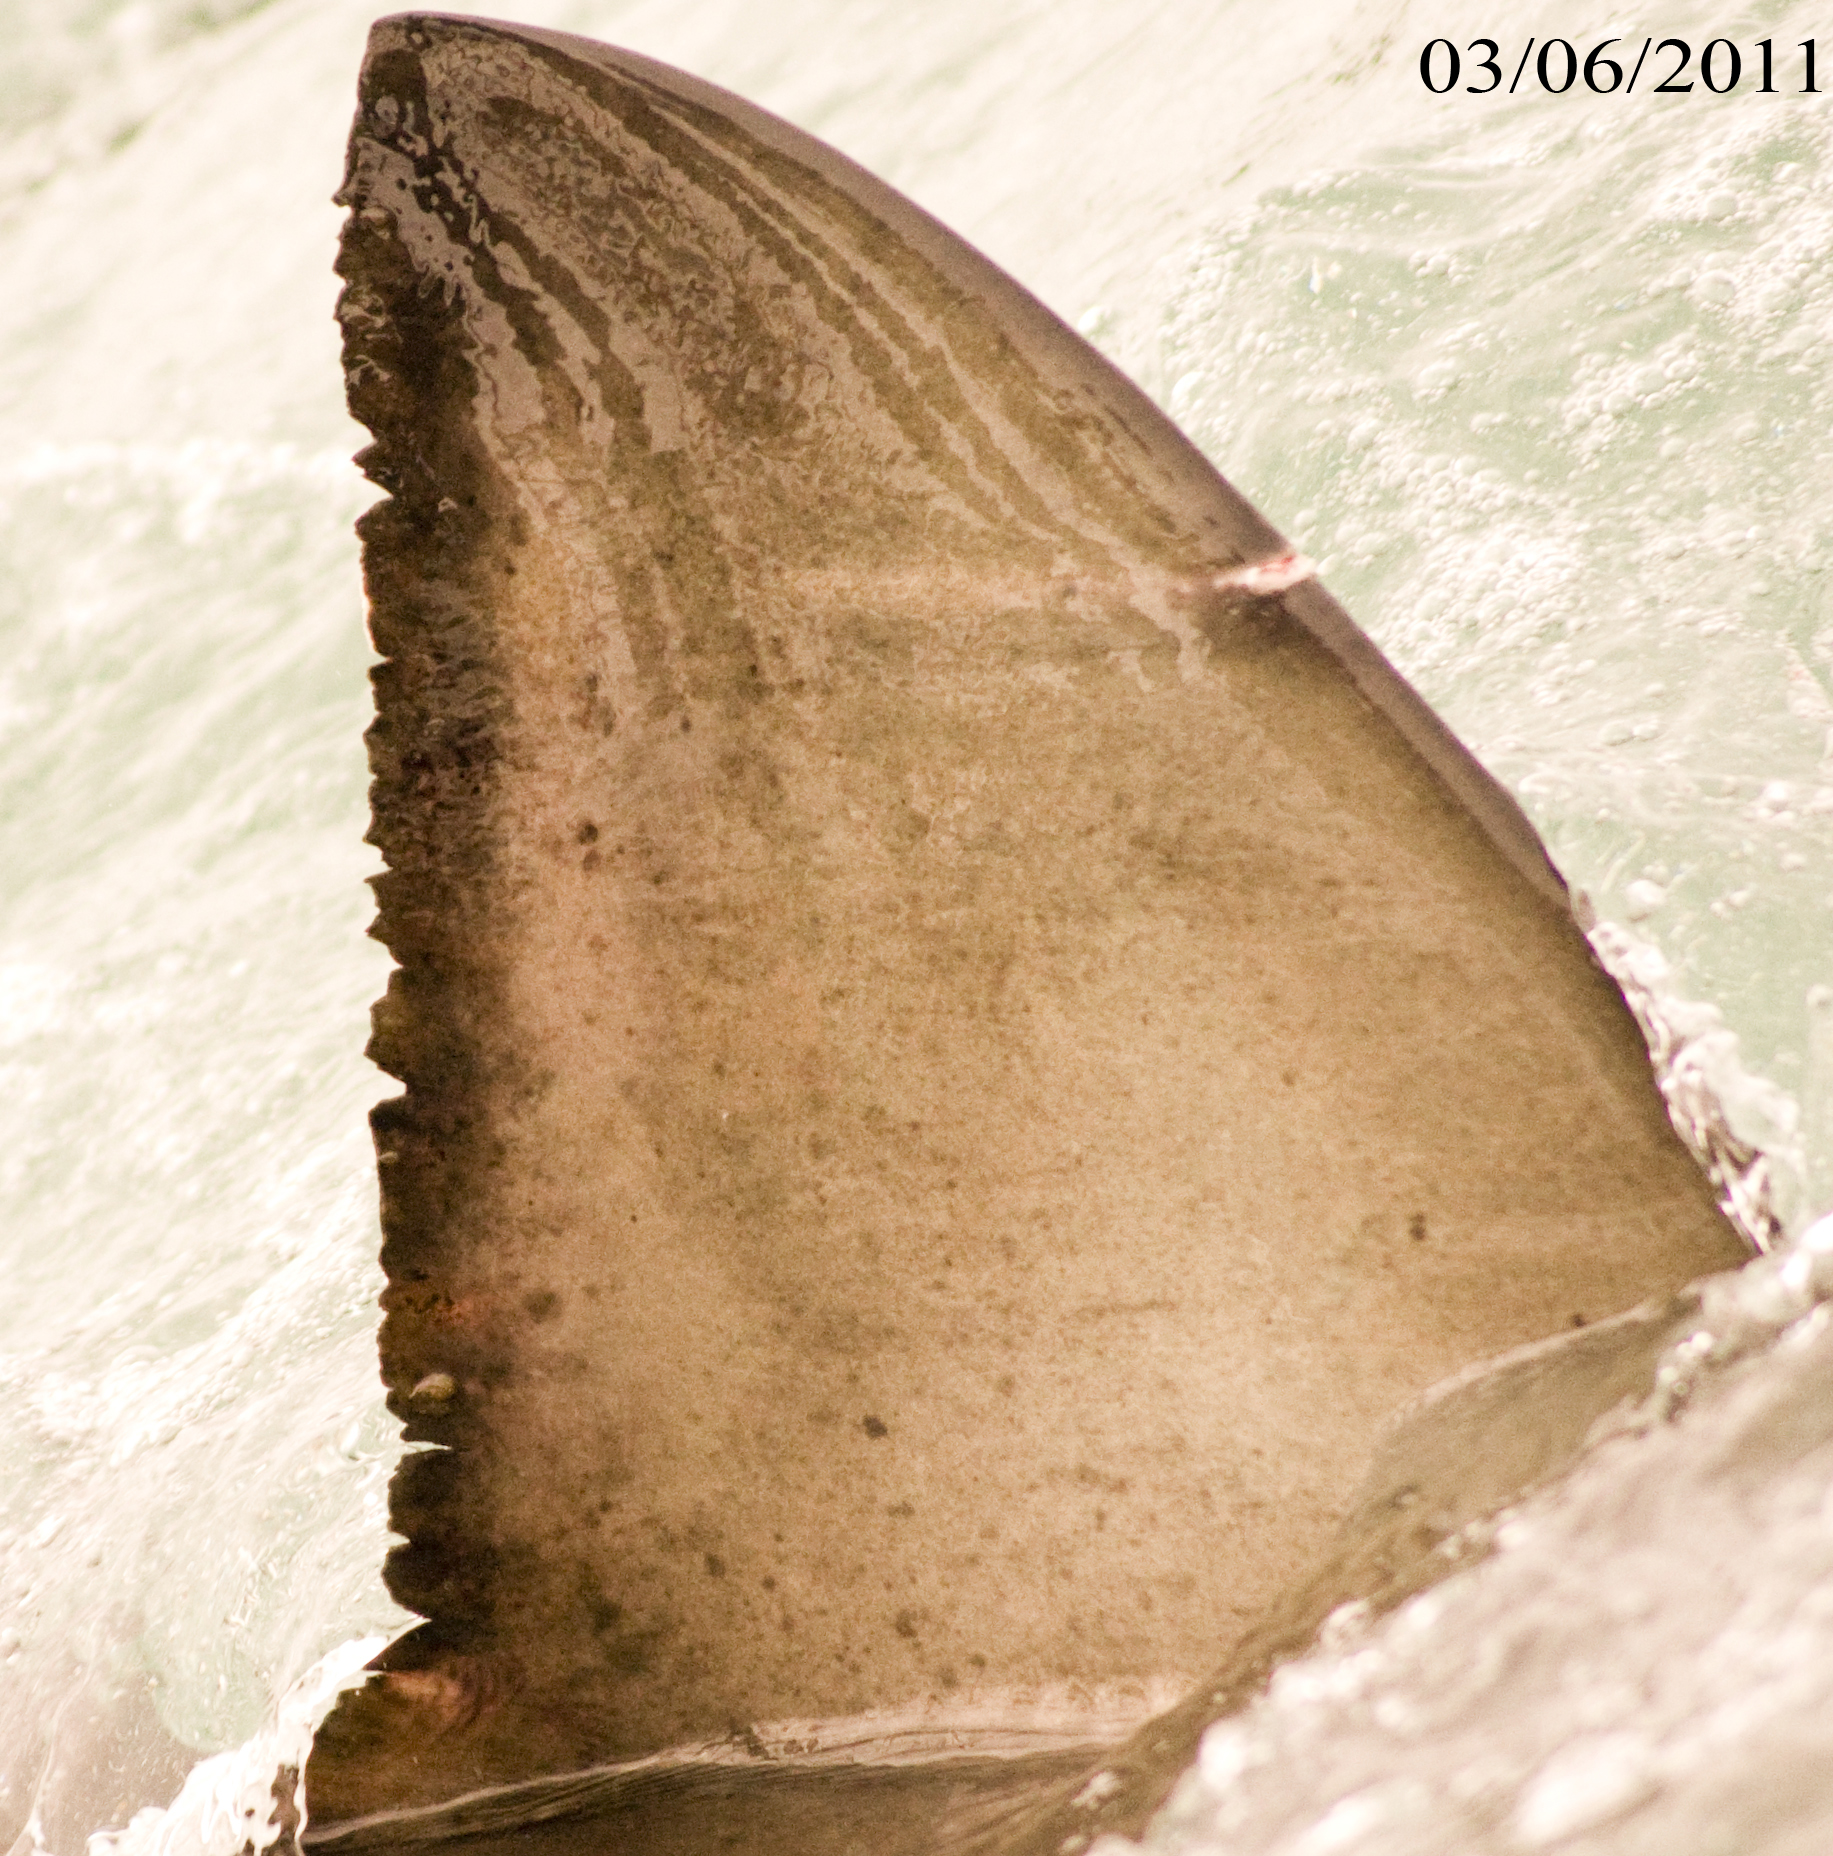
\includegraphics[width=2in]{haai3.jpg}}}
\caption{Fins corresponding to the the same shark.}
\label{gradient}
\end{figure}

This is a problem since those sequences are too far apart for the DTW algortihm
to recognise them as belonging to the same shark.  We apply a simple
transformation to either one of the sequences such that they fit on top of each other
as best as possible, when viewed as a plotted path.
We do this for every pair of sequences compared.  \\
 
A distance matrix, $A_ij$, is then calculated, containing the distance between
each pair of elements,  $dist(\bf{x}_i, \bf{y}_j)$, in the array as entries.
We now view this matrix as a
grid, where the
aim is to find a lowest cost path from the top left corner of the grid to the bottom right
corner of the grid, thereby making sure that each element in the array is compared to every other element in the array.
The minimum cost is then a measure of the similarity between the
sequences.  \\

Thus for a database containing $N$ shark fin images, a $N \times N$ cost
matrix will be returned, where the entry in $(i, j)$ corresponds to the cost
of the path when shark fin $i$ is compared to shark fin $j$.  We then identify the shark
corresponding to the minimum of these entries in a specific
column.
In other words, the lower the cost, the less the sequences differ and the greater the match.  \\

Below is an example where two arrays are compared using DTW. Note the lines
connecting the points being compared.  

\begin{figure}[H]
 \centering
 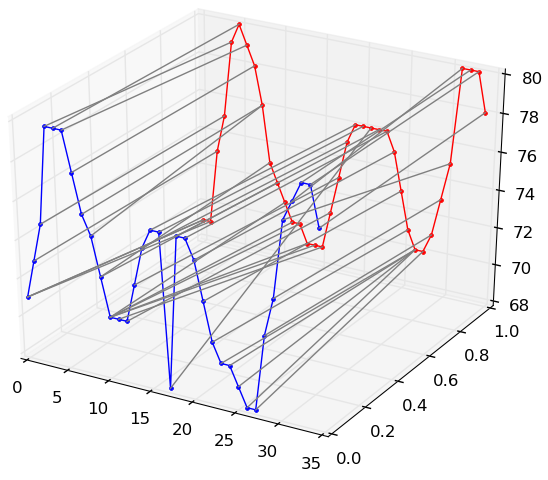
\includegraphics[width=3in]{dtw.jpg}
 \caption{Fins compared as arrays, generated by DTW implementation.}
 \label{dtw}
\end{figure}

Figure \ref{dtw1} shows an example of calculating the distance matrix.

\begin{figure}[H]
 \centering
 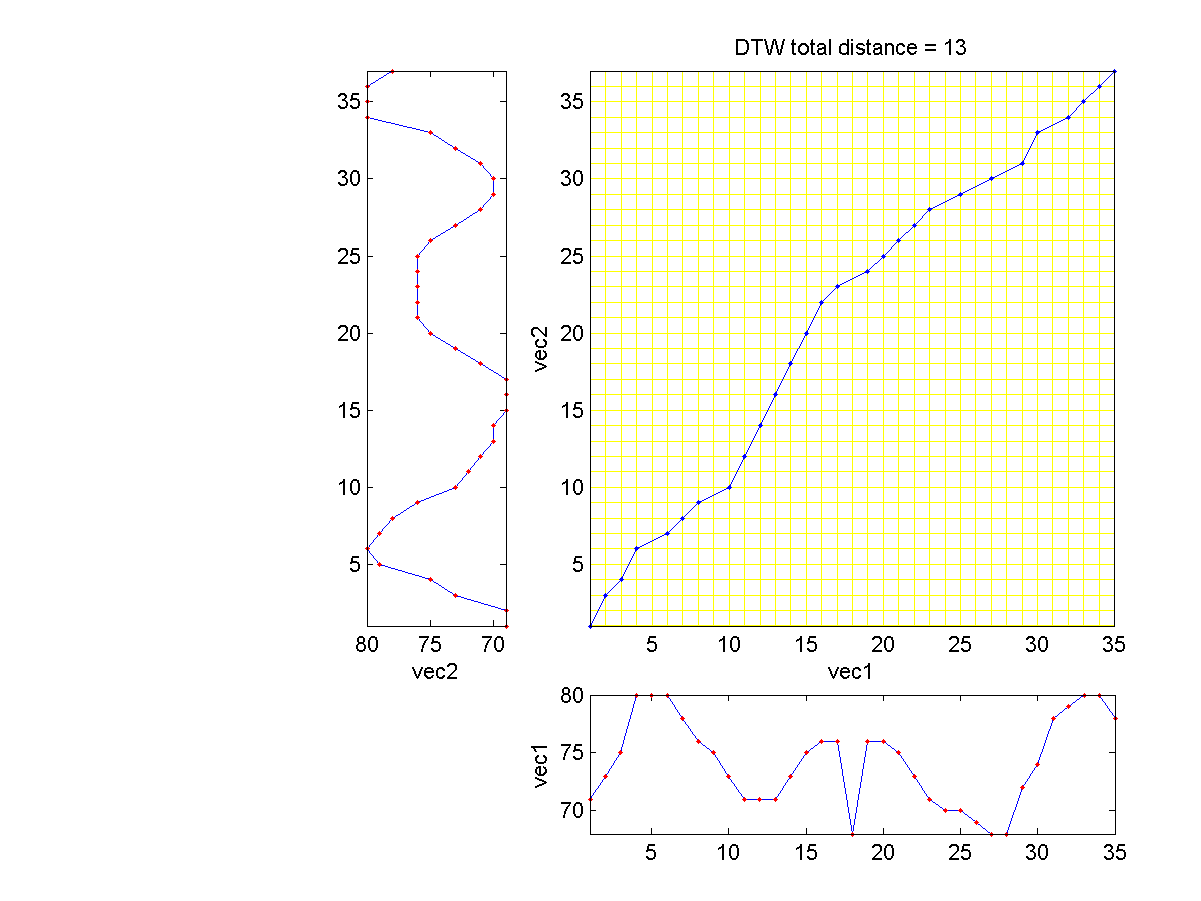
\includegraphics[width=3.5in, height=3in]{dtw1.png}
 \caption{Calculating the distance matrix\cite{dtw}.}
 \label{dtw1}
\end{figure}

For this part of the pipeline, the output from the fin detection method, i.e.
the coordinates of the path defining the shark fin, is used as input.  The DTW
method will follow the above procedure to compare every shark fin to every
other shark fin in the database, each time returning a minimum cost.  \\

\subsection{DARWIN -- Alternative software}
The DARWIN\cite{Darwin} software package is well known when it comes to
aquiring important information about dolphins.  It was initially implemented
by an undergraduate student of
Eckerd College.
Lately it was used to estimate the Great White shark population in the
Gansbaai area by means of shark fin identification and matching.  They claim to
have found approximately
1008 different shark species in this region.  This
claim was tested by Ms. S. Andreotti, using a database of 50 shark fin images and she found that in only
54\% of the cases, the correct matching took place, making this software
unreliable for this specific purpose without further adjustment.

\begin{figure}[H]
 \centering
 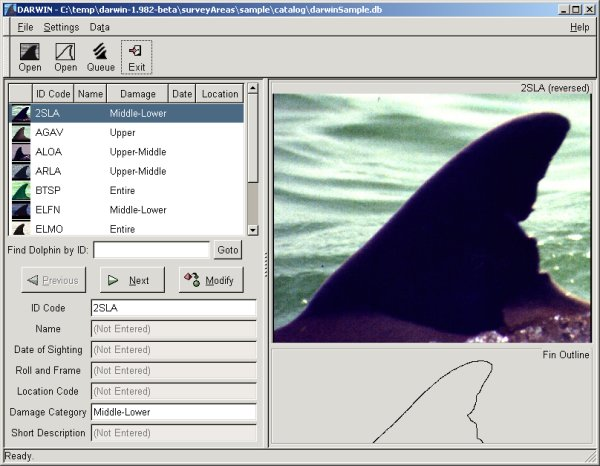
\includegraphics[width=3in]{Darwin.jpg}
 \caption{DARWIN user interface. \cite{Darwin}}
\end{figure}

In this research project, we test our software on the same set of 50 shark fin
images to compare results more effectively.
Since our software is specifically aimed at the identification of sharks, a first attempt at identification will at least 
give a lower bound for the success of our software. \\

In the next section segmentation algorithms are discussed.  

\newpage
\section{Segmentation Algorithms}
\subsection{Different categories and techniques}
Segmentation algorithms can be arranged into different categories. 
Some of the most well-known categories are
\begin{itemize}
 \item \textbf{Thresholding}\cite{threshold}  Thresholding is an unsophisticated method. It
relies on
     selecting a good threshold
     value, using Otsu's method for example, to convert a gray-scale image into
a binary image.  Segmentation is
     then done on the binary image. 
 \item \textbf{Clustering} For these methods, the $K$-means algorithm
can be used to partition an image into $K$ clusters, whereafter
segmentation will follow.
 \item \textbf{Compression-based}\cite{compression} This method conjectures that the
optimal segmentation is the one that minimizes, when considering all possible
segmentations, the coding length of the data; in other words, the number of bits
required to encode that image, based on the given segmentation.
 \item \textbf{Histogram-based}\cite{threshold}  A histogram of 
the image is computed whereafter the peaks and valleys in the histogram
are used to locate clusters in the image.  Here clusters refer to pixels
sharing a certain image property, where the colour or intensity of the pixels can be used
to
locate clusters.
 \item \textbf{Edge detection}\cite{edge} Edge detection is well researched in image
processing.  Region boundaries and edges are closely related,
since there are usually a sharp adjustment at region boundaries.  Edge detection
techniques can therefore be used as a bases for different segmentation
algorithms.
 \item \textbf{Region growing}\cite{threshold} Region merging means taking an initial 
 over-segmentation,
obtained using e.g. SLIC, and then merging those regions based on a set of
pre-determined properties, to form larger segments.  The process
terminates once all pixels are assigned to a specific region.  
 \item \textbf{Watershed transformation} See description in \ref{watershed}.    
 \item \textbf{Graph partitioning}\cite{rw} This method is based on modelling
the image as a weighted, undirected graph, where the nodes represent the pixels
and the weights represent the similarity between neighbouring pixels. Then the
graph is partitioned into clusters according to a specified criterion.  Each
partition is then considered a segment in the image.
 \item \textbf{Trainable}\cite{trainable} Also known as Neural network segmentation,
this process involves processing the small areas of an image by means of an
artificial neural network or a set of neural networks.  Thereafter, using the
categories recognised by the network, the decision-making mechanism marks the
image accordingly and segmentation is done.
\end{itemize}

Waar moet ek hierdie sit??????
The semantic segmentation
algorithm is based on pixel wise object segmentation.  This is done by 
assigning category labels to a set of super pixels obtained by clustering the
joint colour space and coordinate space using the mean shift algorithm.
The method of interactive semantic segmentation as in \cite{RF} can be described
as follows.  Each image is presented as a set of super pixels, where 
a super pixel is a set of pixels.  The first image in the data set must be
segmented manually by labelling each super pixel. An appearance model is 
now created.  The next image is now segmented automatically using the appearance
model.  During the segmentation the user may correct mistakes by 
relabelling and thus updating the appearance model.  Every time the user
approves the segmentation, the system learns from the new labelling information.
As image segmentation continues, user time spent on correcting labels reduces
and thus the rate of image labelling increases. \\

This method can be helpful in the sense that it works with a database of images
of the same kind.  Since the shark fin images are all of the same type, 
it would be very beneficial to manually segment the first image only and then
automatic segmentation will follow.  By updating the appearance model, 
better segmentation results will be obtained.  \\ 

\subsection{Cellular automaton}
\label{ca}
The idea of an cellular automaton is explained with the use of an example.
Probably the most well-known example of a two dimensional automaton is Conway's
Game of Life\cite{gol}, developed by British mathematician John Horton Conway in 1970. 
This "game" is a zero-player game, i.e. it developes according to an initial
state
and requires no further input.  The "player" interacts by creating an initial
state whereafter evolution of cells take place.  \\

The  space in  which the  game  takes place  can  be described  as an  infinite
two-dimensional square grid of cells.  Each cell can
be in one of two states, dead  or alive.  In Conway's Game of Life, each
cell   interacts  with   the  cells   in  its   eight-neighbourhood  or   Moore
neighbourhood.  The following  rules are used to update the state of each cell.
Note that these rules will differ for each automaton.

\begin{itemize}
 \item  Any living cell with less than two living neighbours, will die because of under population.
 \item Any living cell with two or three living neighbours lives on to the next generation.
 \item Any living cell with more than three living neighbours dies because of over population.
 \item Any dead cell with exactly three living neighbours becomes a living cell, because of reproduction.
\end{itemize}

New generations are created by applying these rules simultaneously to every cell and therefore births and deaths occur simultaneously. \\

Below is an example of structures created by
different rules and different initial conditions, all following the procedure described above. \\

\begin{figure}[H]
\centering
\mbox{\subfigure{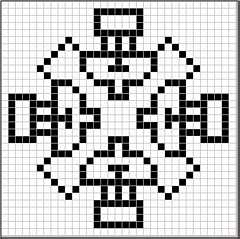
\includegraphics[width=2in]{conway2.jpg}} \quad
\subfigure{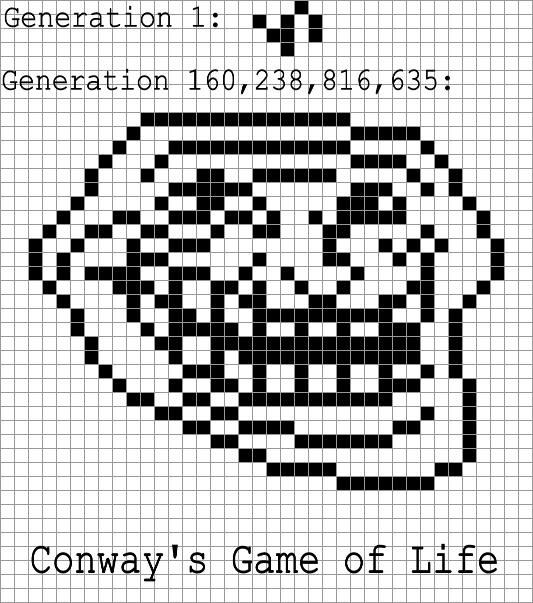
\includegraphics[width=2in]{conway1.png}}}
\caption{Some interesting patterns formed by different cellular automaton\cite{conway}.}
\end{figure}

\subsection{Growcut--Proposed method}
\label{growcut}
The Growcut algorithm is an interactive, multi-label segmentation algorithm
for N-dimensional images.  The algorithm is based on cellular automata, i.e.,
the user labels a few pixels, called the seed pixels, and the rest of the image is then segmented
automatically by a cellular automaton as described in \ref{ca}. 
A new generation of cells is then created according to a fixed rule or
mathematical function that determines the new state of the cell, by looking at
the current state of the cell as well
as that of its neighbourhood.  Two of the most common neighbourhood systems used are the Von
Neumann neighbourhood and the Moore neighbourhood which are shown below. \\

\begin{figure}[H]
\centering
\mbox{\subfigure{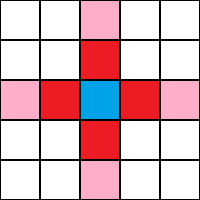
\includegraphics[width=1.7in]{VonNeumann.png}} \quad
\subfigure{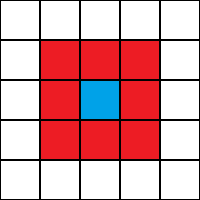
\includegraphics[width=1.7in]{Moore.png}}} \caption{Von Neumann and
Moore neighbourhood systems\cite{n}.}
\end{figure}

The algorithm is interactive, since the user can observe the segmentation and
guide the algorithm in places where the segmentation is difficult to compute.
\\

\noindent We now explain the basic method\cite{alg}.  A
cellular automaton is an algorithm which is discrete in both space and time
and operates on a lattice of pixels $p \in P \subset Z^{n}$.  A cellular
automaton can be considered as a triplet, $A = (S, N, \delta)$, where $S$ is a
set containing different states, $N$ is the
neighbourhood system of the cell and $\delta: S^{N} \rightarrow S $ is a
transition rule.  This is the function which defines  the rule calculating the
cell's state at time $t + 1$, given the states 
of the cell's neighbourhood at time $t$.  In this research project, the Moore 
Neighbourhood system is used.  The cell state referred to
is also
considered a triplet $(l_{p}, \theta_{p}, \overrightarrow{C}_{p})$.
$l_{p}$ is the label of the cell, either foreground or background in this case, $\theta_{p}$ is the
'strength' of the cell, or in other words the certainty that the cell is either foreground or background and $\overrightarrow{C}_{p}$ is
the cell feature vector, depicting the difference in intensity values between two cells.  Without loss of generality it can be assumed that
$\theta_{p} \in [0,1]$.  \\

The initial state of the pixels is set to $l_{p} = 0, \theta_{p} = 0,
\overrightarrow{C}_{p} = RGB_{p}$, where $RGB_{p}$ is a three dimensional vector
of the pixel's colour in 
the RGB space.  The goal of the segmentation is to assign one of the possible
$K$ labels to each one of the pixels.  The user starts the segmentation by
marking specific pixels as foreground and others as background.  This sets the
initial state of each pixel.  While the labels are being updated, the user can
correct and guide the process if desired.  \\

\noindent The pseudo code for the automata evolution rule is shown\cite{alg}.
\begin{algorithm}[H]
\begin{algorithmic}[1]
 \State // For each cell...
 \For{$\forall p \in P$}
 \State // Copy previous state
 \State $l^{t+1}_{p} = l^{t}_{p}$;
 \State $\theta_{p}^{t+1} = \theta_{p}^{t}$;
 \State // Neighbours try to attack the current cell
 \For{$\forall q \in N(p)$}
 \If{$g(\| \overrightarrow{C}_{p} - \overrightarrow{C}_{q} \|_{2}) \cdot
\theta^{t}_{q} > \theta_{p}^{t}$}
 \State $l^{t+1}_{p} = l^{t}_{q}$
 \State $\theta^{t+1}_{p} = g(\| \overrightarrow{C}_{p} - \overrightarrow{C}_{q}
\|_{2}) \cdot \theta^{t}_{q}$
 \EndIf
 \EndFor
 \EndFor
\end{algorithmic}
\end{algorithm}

\noindent where $g$ is a monotonous decreasing function bounded to $[0, 1]$. 
The function is given by
\[
g(x) = 1 - \frac{x}{max\| \overrightarrow{C} \|_{2}}. 
\]\\

We now supply an intuitive explanation of the above.
The Growcut algorithm takes the following parameters: an N-dimensional input image,
an initial state, which stores (foreground/background, strength) for
each pixel position or automaton.  The strength represents the
certainty of the state (e.g., 1 is a hard seed value that remains
constant throughout segmentation), the maximum number of automata iterations to allow   
(the segmentation may complete earlier if the state no longer varies) and the
size of the neighbourhood window.  The algorithm will return a segmented image, 
where a value of zero indicates background and a value of one indicates foreground. \\

It can be helpful to view the labelling process as ongoing growth and struggle of $K$ different species.
The species start to "grow" from the seeded pixels, trying to occupy the whole image.  
Each iteration involves every cell trying to "attack" its neighbour, cell $q$ "attacking" cell $p$ for instance. 
The strength of the attack is determined by the attacker's cell strength, $\theta_{q}$, and
the difference in intensity values of $p$ and $q$. \\

Whenever the attack strength is greater than the defend strength, the defending cell is "conquered" and
its strength and label is updated to that of the attacker. 
These iterations continue until either the maximum number of iterations is met or the automaton has converged,
where cell state seize to change.  Note that convergence is guaranteed since cell strength is increasing and bounded. \\

\noindent The algorithm is modified in the following way.  One of the
main features that needs attention is the damping function $g$.  By changing
the exponent of the term $\frac{x}{max\| \overrightarrow{C} \|_{2}}$ to
$\frac{3}{2}$, thus $\left ({\frac{x}{max\| \overrightarrow{C} \|_{2}}}\right
) ^\frac{3}{2}$,
an immediate result was seen.  Since the edges of the shark fin now 
  had a higher value, the algorithm was less likely to cross them. \\  
 
Figures \ref{fin1} and \ref{fin2} show a comparison between the result of the original algorithm on
one of the shark fin images and the effect of the modified version of the
algorithm on the same image.  The green and red markers indicate the selected foreground and background pixels respectively.

\begin{figure}[H]
 \centering
 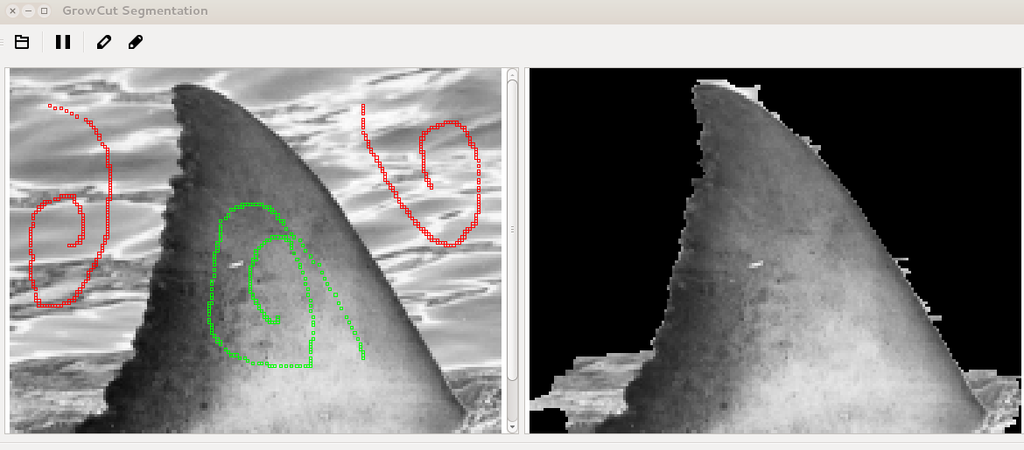
\includegraphics[width=4in, height=1.8in]{haaio}
 \caption{The effect of the original algorithm}
 \label{fin1}
\end{figure}

\begin{figure}[H]
 \centering
 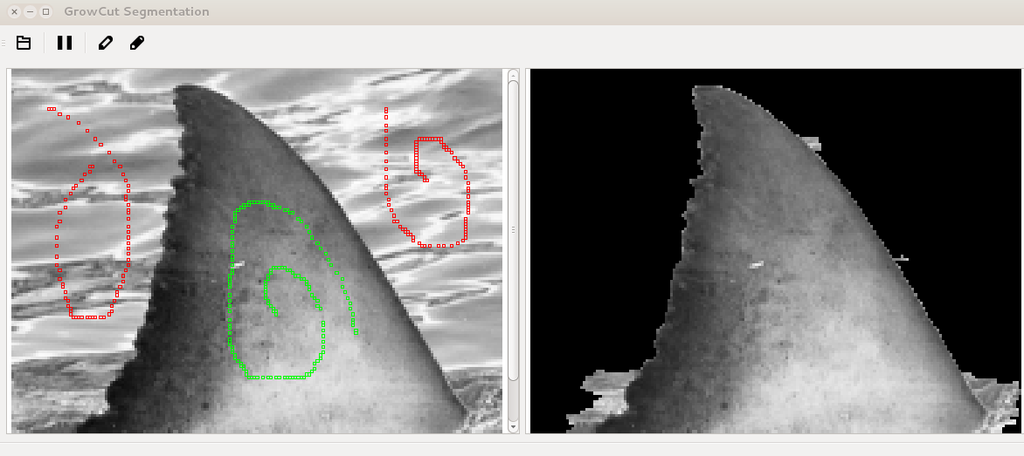
\includegraphics[width=4in, height=1.8in]{haaim}
 \caption{The effect of the modified algorithm}
 \label{fin2}
\end{figure}

\noindent It can be seen that the modified version gives better results around
the edges, which is essential in the case of the shark fin images. \\  


\subsection{Random Walker}
This method, as
described in \cite{rw}, is as follows.  The user labels a few
pixels as foreground or background for example.  This is then called the seeds. 
A random walker is then released from each of the unlabelled pixels. 
Thereafter, the probability that a certain pixel's random walker first arrives
at a specific seed, is computed.  The latter is done by modelling the image as a weighted graph, where
the weight of an edge reflects the similarity (intensity values) between pixels,
and then solving a system of linear equations.  The pixel is then assigned the
label
of the seed for which it is most likely to reach.  The process is repeated until
each pixel is assigned a specific label.


\subsection{Watershed}
\label{watershed}
Another segmentation algorithm is the classic watershed algorithm, as
implemented in \cite{scikit}.  If the image is viewed
  as a landscape, the seed points or user defined markers are viewed as the locations of water sources.  The algorithm then floods
basins from the user-defined markers until basins which attribute to different
markers meet at watershed lines.  In this case marker positions are chosen as
the local maxima of the image.  Thereafter the segmentation is done on the
gradient image.  The result of the watershed algorithm applied to a shark fin
image is shown in Figure \ref{fig3}.

\begin{figure}[H]
\centering
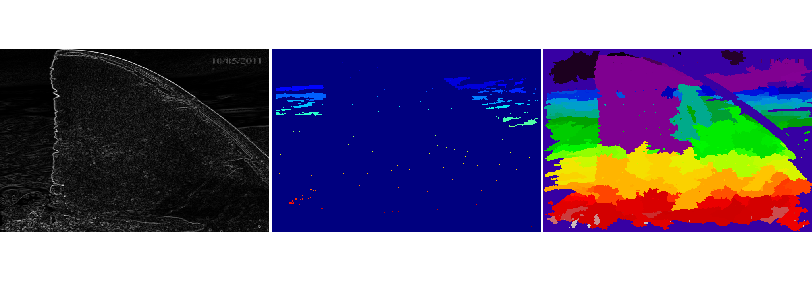
\includegraphics[width=5in,height=2in]{watershed.png} 
\label{fig3}
\caption{The watershed algorithm\cite{scikit}.}
\end{figure}

\noindent The first image shows the gradient image of the original shark fin
image.  The second image shows the pixels that are identified as a local maxima.
 The third image shows how the basins flooded until watershed lines are reached.
 By joining the correct segments, an effective segmentation can be performed -- this however will require
 a lot of hard work.

\newpage
\section{Results}
\subsection{}


\subsection{}


\newpage
\section{Conclusions}
This research project entailes studying different segmentation algorithms with the idea to be able to identify sharks for various environmental and biological reasons.
A request from a PhD student for assistance in her research project on identifying sharks led to the development of a pipeline. The Growcut algorithm is used as the main segmentation algorithm. A workable pipeline is developed. \\

\subsection{Future work}
Future work entails developing a user
interface, making the identification of shark fins more user friendly and interactive.
An user, who must be connected to some database of shark fins, will be able to
use this interface, acting as a front end to the
  pipeline, to identify shark fins.  The
results from the different sections of the pipeline can be
  inspected individually, in
conjunction with each other or as a whole.  New shark fin images can then be
uploaded, from which statistical queries and reports can be
made from the database. \\

For example, the segmentation window will allow the user to manually select foreground and background pixels as described in \ref{segmentation}.
When performing the algorithm, the user can guide the process by selecting more pixels for segmentation. \\

Another aspect that needs investigation is the fact that the algorithms are not
running at optimum speed.  Cython can be considered
as a potential remedy. \\

One can also investigate the various parameters in the Growcut algorithm, like the window size, the damping function and attacking strategies. \\

After the classification of shark fins is done, it would be valuable if different sharks could be "clustered" according to fin similarities.
Recognizing various families of sharks can then be attempted.  Updating the database to include information about sharks can be valuable to marine biologists.  \\

\newpage
\bibliography{final}

\end{document}
